\documentclass[11pt]{article}

\usepackage[margin=2.5cm]{geometry}
\usepackage{graphicx}
\usepackage{float}
\usepackage{graphicx}
\restylefloat{figure}

\title{Your Title}
\author{Your Name}
\date{\today}


\begin{document}

\maketitle
\pagebreak

\section{Introduction}
An arithmetic logic unit (ALU) is a multi-operation, combinational-logic digital function. It can 
perform a set of basic arithmetic operations and a set of logic operations. The ALU has a number of selection lines to select a particular operation in the unit. The selection lines are decoded 
within the ALU so that k selection variables can specify up to $2^k$
distinct operations.


Figure 1 shows the block diagram of a 4-bit ALU. The four data inputs from A are combined with the four inputs from B to generate an operation at the F outputs. The mode-select 
input $s_2$ distinguishes between arithmetic and logic operations. The two function-select inputs $s_1$
and $s_0$ specify the particular arithmetic or logic operation to be generated. With three selection 
variables, it is possible to specify four arithmetic operations (with $s_2$ in one state) and four logic 
operations (with $s_2$ in the other state). The input and output carries have meaning only during an 
arithmetic operation.
The input carry in the least significant position of an ALU is quite often used as a fourth 
selection variable that can double the number of arithmetic operations. In this way, it is possible 
to generate four more operations, for a total of eight arithmetic operations.

The input carry in the least significant position of an ALU is quite often used as a fourth 
selection variable that can double the number of arithmetic operations. In this way, it is possible 
to generate four more operations, for a total of eight arithmetic operations.

\begin{figure}[ht]
\centering
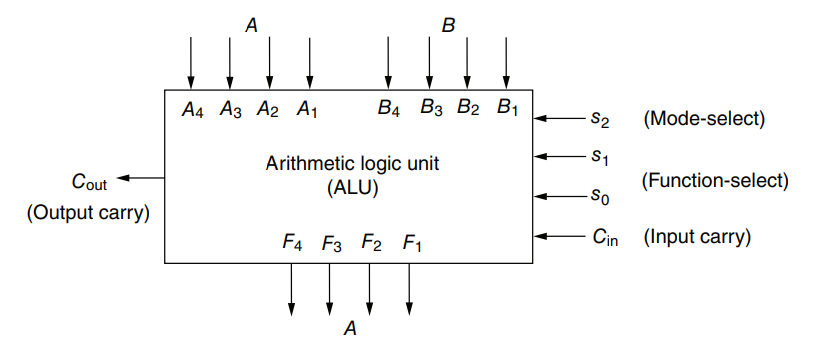
\includegraphics[width=0.9\textwidth]{images/ALU.png}
\caption{Block Diagram of a 4-bit ALU}
\end{figure}

The design of a typical ALU will be carried out in three stages. First, the design of the 
arithmetic section will be undertaken. Second, the design of the logic section will be considered. 
Finally, the arithmetic section will be modified so that it can perform both arithmetic and logic 
operations.

There are also 4 status outputs (flags) in ALU. They are denoted by C(Carry
Flag), Z(Zero Flag), V(Overflow Flag), S(Sign Flag). Their representations carry out the
following meanings:
\begin{itemize}
    \item C(Carry Flag): This flag is set when there is a carry out of the most significant bit of the result.
    \item Z(Zero Flag): This flag is set when the result of the operation is zero.
    \item V(Overflow Flag): This flag is set when the result of the operation is too large to be represented in the given number of bits.
    \item S(Sign Flag): This flag is set when the result of the operation is negative.
\end{itemize}

\section{Problem Specification with assigned instructions}
Design a 4-bit ALU with three selection bits CS2, CS1, CS0 that can perform the following operations:
\begin{table}[ht]
    \centering
    \begin{tabular}{|c|c|c|c|}
        \hline
        \textbf{CS2} & \textbf{CS1} & \textbf{CS0} & \textbf{Functions} \\
        \hline
        0 & 0 & 0 & Add \\
        \hline
        0 & 0 & 1 & AND \\
        \hline
        0 & 1 & X & Sub with borrow \\
        \hline
        1 & 0 & 0 & Complement A \\
        \hline
        1 & 0 & 1 & OR \\
        \hline
        1 & 1 & X & NEG A \\
        \hline
    \end{tabular}
    \caption{Control Signals and Functions of the 4-bit ALU}
\end{table}

Here, CS2, CS1, and CS0 are the control signals. X means that the value of the signal is not important. The ALU should have 4 status outputs (flags) C, Z, V, S.
\begin{figure}[ht]
    \centering
    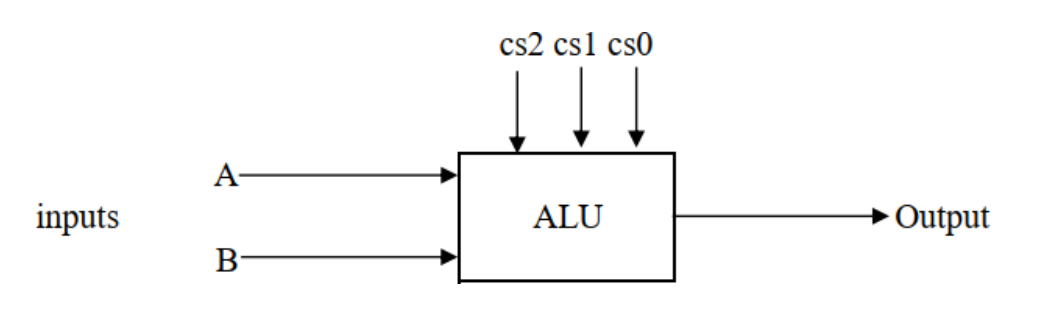
\includegraphics[width=0.9\textwidth]{images/ALU2.png}
    \caption{Block Diagram of a 4-bit ALU}
\end{figure}

\section{Detailed design steps with k-maps (if applicable)}

\section{Truth Table}
\begin{table}[ht]
    \centering
    \begin{tabular}{|c|c|c|c|c|c|c|c|c|c|c|}
        \hline
        CS2 & CS1 & CS0 & Functions & X & S11 & S10 & Y & $\bar{\textnormal{E2}}$ & S2 & Cin \\
        \hline
        0 & 0 & 0 & Add & A & 0 & 0 & B & 0 & 0 & 0 \\
        \hline
        0 & 0 & 1 & AND & AB & 0 & 1 & 0 & 1 & X & 0 \\
        \hline
        0 & 1 & X & Sub with borrow & A & 0 & 0 & B' & 0 & 1 & 0 \\
        \hline
        1 & 0 & 0 & Complement A & A' & 1 & 0 & 0 & 1 & X & 0 \\
        \hline
        1 & 0 & 1 & OR & A+B & 1 & 1 & 0 & 1 & X & 0 \\
        \hline
        1 & 1 & X & NEG A & A' & 1 & 0 & 0 & 1 & X & 1 \\
        \hline
    \end{tabular}
    \caption{Truth Table of the 4-bit ALU}
\end{table}

\section{Block Diagram}

\section{Complete Circuit Diagram}

\section{ICs used with count as a chart}
\begin{table}[ht]
    \centering
    \begin{tabular}{|c|c|}
        \hline
        IC & Count \\
        \hline
        74153 & 2 \\
        \hline
        74157 & 1 \\
        \hline
        7408 & 2 \\
        \hline
        7432 & 2 \\
        \hline
        7404 & 2 \\
        \hline
        7486 & 1 \\
        \hline
        7483 & 2 \\
        \hline
    \end{tabular}
\end{table}

\section{The simulator used along with the version number}

\section{Discussions}

\section{Contribution of Each Member}

\end{document}
